% !TEX root = ../rampMeteringViaTheAdjoint.tex
\def \scale{1.5}
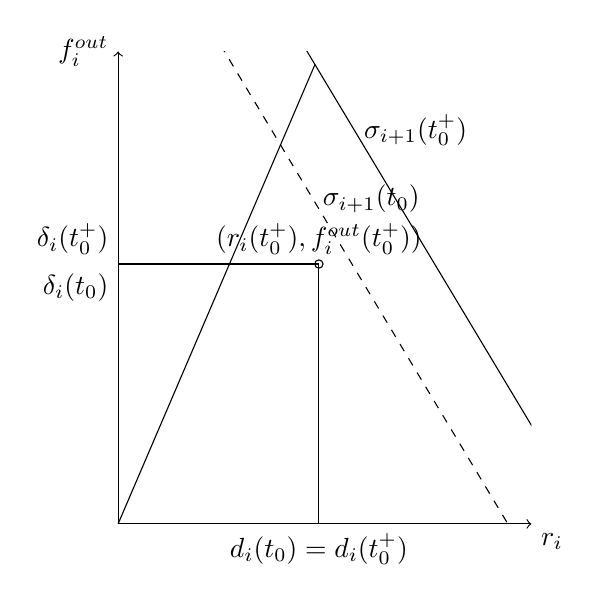
\begin{tikzpicture}[scale=\scale,domain=0:1]

\def \rampDem{1.7}
\def \dem{2.2}
\def \priorityRat{0.7}
\def \splitRat{0.4}
\def \totalFlow{3.3}
\def \totalFlowPlus{4}

\coordinate (Z) at (0,0);
\coordinate (I1) at (\rampDem, 0);
\coordinate (I2) at (0, \dem);
\coordinate (I3) at (\rampDem, \dem);

\coordinate (A) at (0, {\totalFlow/(1-\splitRat)});
\coordinate (B) at (\totalFlow, 0);
\coordinate (A') at (0, {\totalFlowPlus/(1-\splitRat)});
\coordinate (B') at (\totalFlowPlus, 0);

\coordinate (C) at ({(1-\priorityRat)/\priorityRat*\dem}, \dem);
\coordinate (D) at (intersection of A'--B' and Z--C);
\coordinate (E) at (\rampDem, \dem);


\draw[->] (Z) -- (3.5,0) node[below right]{$r_i$};
\draw[->] (Z) -- (0,4) node[left]{$f^{\text{out}}_i$};

\draw (I3) -- (I1) node[below]{$d_i(t_0) = d_i(t_0^+)$};
\draw (I3) -- (I2) node[below left]{$\delta_i(t_0)$} node[above left]{$\delta_i(t_0^+)$};

\begin{scope}
\clip (Z) rectangle (3.5, 4);
\draw[dashed] (A) -- (B) node[midway, right]{$\sigma_{i+1}(t_0)$};
\draw (A') -- (B') node[midway, right]{$\sigma_{i+1}(t_0^+)$};
\end{scope}

\draw (Z) -- (D) node[midway, xshift=1cm]{};
\draw (E) circle (1pt) node[above]{$(r_i(t_0^+), f_i^{\text{out}}(t_0^+))$};

\end{tikzpicture}